\documentclass[conference]{IEEEtran}

\usepackage{cite}
\usepackage{amsmath,amssymb,amsfonts}
\usepackage{graphicx}
\usepackage{booktabs}
\usepackage{multirow}
\usepackage{array}
\usepackage{url}
\usepackage[hidelinks]{hyperref}
\usepackage[caption=false,font=footnotesize]{subfig}
\usepackage{stfloats}
\usepackage{placeins}
\usepackage{algorithm}
\usepackage{algpseudocode}
\sloppy

\begin{document}

\title{Retina-Aware Explanation Consistency Scoring for Reliable Diabetic Retinopathy Classification}

\author{
\IEEEauthorblockN{
Mrigank Jaiswal,
Pranav,
Nanevarth Prakash
}

\IEEEauthorblockA{
Department of Electronics and Communication Engineering (DoECE)\\
Central University of Jammu, India\\
Email: 23beece10.ece@cujammu.ac.in
}
}

\maketitle

\begin{abstract}
Automated diabetic retinopathy (DR) screening systems must be accurate, but in real clinical use they must also be reliable, calibrated, and interpretable. A model that produces a correct label with poorly calibrated confidence or anatomically inconsistent attention remains difficult to trust in safety-critical settings. This paper presents a retina-aware reliability framework for DR classification from retinal fundus images. An EfficientNet-B0 classifier is trained on the APTOS dataset and post-hoc calibrated using temperature scaling to improve the quality of predictive probabilities. To move beyond confidence-only reliability estimation, this work introduces a retina-aware Explanation Consistency Score (ECS) that combines calibrated confidence, predictive entropy, Grad-CAM focus, and spatial overlap between Grad-CAM attention maps and the retinal region. The resulting score is used for selective prediction, enabling the system to accept only sufficiently reliable outputs.

Experimental results show that temperature scaling improves reliability without changing classification accuracy, reducing Expected Calibration Error (ECE) from 0.0635 to 0.0411. The proposed retina-aware ECS further improves selective prediction over a confidence-only baseline. At a threshold of 0.5, the proposed method achieves 81.82\% coverage with 86.00\% selective accuracy, compared with 86.18\% coverage and 82.70\% selective accuracy for confidence-only selection. At a stricter threshold of 0.7, the proposed framework reaches 94.14\% selective accuracy at 55.82\% coverage. These results demonstrate that integrating explainability with anatomical consistency provides a more reliable basis for trustworthy medical image classification.
\end{abstract}

\begin{IEEEkeywords}
Diabetic retinopathy, calibration, Grad-CAM, explainable AI, selective prediction, reliability, medical image classification
\end{IEEEkeywords}

\section{Introduction}
Diabetic retinopathy (DR) is one of the major causes of preventable blindness worldwide, and timely diagnosis remains critical for reducing irreversible vision loss. As retinal screening programs continue to scale, automated fundus image analysis has emerged as an important application of artificial intelligence in healthcare. Deep learning methods, especially convolutional neural networks, have shown strong promise in DR grading from retinal fundus images. However, high classification accuracy alone is not sufficient for practical deployment in medical decision-making systems.

In safety-critical settings, the output of a model must be not only accurate but also trustworthy. A neural network may assign a high confidence score to a wrong prediction, or it may reach the correct decision for the wrong visual reason. Such behavior is problematic in medical imaging, where decisions must be explainable and aligned with clinically meaningful evidence. Calibration methods improve the agreement between predicted probabilities and true correctness, but they do not reveal whether a model is attending to anatomically valid regions. Conversely, explainability tools such as Grad-CAM provide spatial insight into the model’s reasoning, but they are usually used only for qualitative analysis rather than as an active reliability signal.

This work addresses these limitations by proposing a retina-aware Explanation Consistency Score (ECS) for reliable diabetic retinopathy classification. The central idea is that a trustworthy prediction should satisfy multiple conditions simultaneously: it should be confident, low in uncertainty, visually focused, and anatomically consistent with the retinal region. To implement this idea, the proposed framework combines calibrated confidence, predictive entropy, Grad-CAM focus, and overlap between Grad-CAM activations and a retinal mask. The score is then used within a selective prediction setting, allowing the model to accept reliable cases and defer uncertain ones.

The main contributions of this paper are as follows:
\begin{itemize}
    \item A calibrated deep learning pipeline for diabetic retinopathy classification using retinal fundus images.
    \item A retina-aware Explanation Consistency Score that integrates confidence, entropy, Grad-CAM focus, and retinal overlap into a single reliability score.
    \item A selective prediction framework that improves trustworthiness compared with a confidence-only baseline.
    \item A quantitative and qualitative evaluation on the APTOS dataset showing improved risk--coverage trade-offs and more reliable accepted predictions.
\end{itemize}

\section{Related Work}
Deep learning for diabetic retinopathy detection has been widely explored using convolutional neural networks and transfer learning. Public retinal datasets such as APTOS and EyePACS have enabled the development of automatic DR grading systems with strong classification performance. However, a large portion of prior work has primarily emphasized predictive accuracy and quadratic weighted kappa (QWK), while comparatively less attention has been given to calibration, reliability, and selective decision-making.

Model calibration has become an important topic in modern deep learning because predicted confidence often does not match actual correctness. Guo \textit{et al.} showed that modern neural networks can be significantly miscalibrated and proposed temperature scaling as an effective post-hoc calibration method \cite{guo2017calibration}. Ensemble-based approaches have also been shown to improve predictive robustness and uncertainty estimation \cite{lakshminarayanan2017ensembles}. In medical applications, these reliability improvements are particularly valuable because decision errors may have severe clinical consequences.

Explainability has likewise become central in medical AI. Grad-CAM is one of the most widely used visual explanation techniques for convolutional networks, as it highlights class-discriminative image regions that influence the model’s decision \cite{gradcam}. In retinal imaging, such heatmaps can reveal whether a model is attending to relevant retinal structures. Yet in most existing systems, explainability remains a passive visualization layer and is not explicitly incorporated into the reliability estimation process.

Selective prediction provides an additional mechanism for safer deployment by allowing a model to abstain on uncertain cases. Confidence-based rejection is a natural baseline, but confidence alone does not always capture whether a prediction is trustworthy. The present work builds on these three strands --- calibration, explainability, and selective prediction --- and unifies them into a retina-aware reliability framework.

\section{Proposed Framework}

\subsection{Problem Formulation}
Let $x \in \mathbb{R}^{H \times W \times 3}$ denote a retinal fundus image, where $H$ and $W$ are the image height and width, respectively, and the final dimension corresponds to the three RGB color channels. Each image is associated with a diabetic retinopathy severity label $y \in \{0,1,2,3,4\}$, where the five classes represent increasing severity of disease progression.

A deep neural network parameterized by $\theta$, denoted by $f_\theta(\cdot)$, maps the input image $x$ to a vector of logits:
\begin{equation}
\mathbf{z} = f_\theta(x), \quad \mathbf{z} \in \mathbb{R}^{C},
\end{equation}
where $C=5$ is the total number of output classes, and each element $z_i$ denotes the unnormalized score associated with class $i$.

The predicted probability distribution is obtained through the softmax function:
\begin{equation}
p(y_i \mid x) = \frac{\exp(z_i)}{\sum_{j=1}^{C}\exp(z_j)},
\end{equation}
where:
\begin{itemize}
    \item $z_i$ is the logit corresponding to class $i$,
    \item $p(y_i \mid x)$ is the predicted probability of class $i$ given input image $x$,
    \item $C$ is the number of classes.
\end{itemize}

The final class prediction is:
\begin{equation}
\hat{y} = \arg\max_i \, p(y_i \mid x).
\end{equation}

In a conventional classification setting, the output $\hat{y}$ is treated as the final decision. In contrast, the goal of this work is broader: beyond predicting the class label, the model must estimate whether the prediction is reliable enough to be accepted. This transforms the problem into a reliability-aware classification setting, where decision-making depends not only on class probabilities but also on confidence quality, uncertainty, explanation consistency, and anatomical alignment.

\subsection{Dataset and Preprocessing}
The proposed framework is evaluated on the APTOS 2019 Blindness Detection dataset, which contains color retinal fundus images labeled into five diabetic retinopathy severity grades. The dataset reflects realistic challenges encountered in medical imaging, including class imbalance, variations in illumination, black borders, and inconsistencies in acquisition conditions.

To standardize the inputs, black borders surrounding the fundus region were removed using threshold-based cropping. Images were then resized to $224 \times 224$, normalized using ImageNet mean and standard deviation, and augmented during training with horizontal flipping, mild rotation, and controlled color jitter. These transformations were selected to improve generalization while preserving medically relevant retinal structures. A stratified train--validation--test split was used to maintain class proportions across subsets.

\subsection{Backbone Model Selection}
EfficientNet-B0 was selected as the primary classification backbone because it offers a favorable trade-off between predictive performance, computational efficiency, and training stability. Compared with larger architectures, EfficientNet-B0 provides strong feature extraction capacity while remaining efficient enough for repeated experimentation involving calibration, Grad-CAM generation, threshold sweeping, and reliability analysis.

The backbone was initialized with ImageNet pretrained weights to leverage transfer learning. This is particularly useful in medical imaging, where labeled data are comparatively limited. The original classification head was replaced with a five-class linear layer corresponding to diabetic retinopathy grading.

\subsection{Training Objective}
To address class imbalance in the APTOS dataset, the model is trained using class-weighted cross-entropy loss:
\begin{equation}
\mathcal{L}_{CE} = - \sum_{i=1}^{N} \sum_{c=1}^{C} w_c \, y_{ic} \log(p_{ic}),
\end{equation}
where:
\begin{itemize}
    \item $N$ is the total number of training samples,
    \item $C$ is the number of classes,
    \item $w_c$ is the weight assigned to class $c$,
    \item $y_{ic} \in \{0,1\}$ indicates whether sample $i$ belongs to class $c$,
    \item $p_{ic}$ is the predicted probability of class $c$ for sample $i$.
\end{itemize}

The class weights $w_c$ are inversely proportional to class frequency, which increases the contribution of underrepresented categories and prevents the model from being dominated by the most common classes. Optimization is performed using AdamW, which decouples weight decay from gradient updates and improves generalization stability.

\subsection{Calibration Module}
Modern neural networks often produce overconfident predictions, especially in medical imaging tasks where inter-class boundaries may be subtle. To improve the reliability of predicted probabilities, temperature scaling is applied as a post-hoc calibration technique.

Given logits $\mathbf{z}$, the calibrated probabilities are computed as:
\begin{equation}
p(y_i \mid x, T) = \frac{\exp(z_i/T)}{\sum_{j=1}^{C}\exp(z_j/T)},
\end{equation}
where:
\begin{itemize}
    \item $T > 0$ is the temperature parameter,
    \item $z_i$ is the logit of class $i$,
    \item $C$ is the total number of classes.
\end{itemize}

The temperature parameter $T$ is optimized on the validation set by minimizing negative log-likelihood. When $T > 1$, the probability distribution becomes softer, thereby reducing overconfidence. Importantly, temperature scaling preserves the ranking of logits, which means classification accuracy remains unchanged while calibration improves.

\subsection{Explainability via Grad-CAM}
To capture the spatial reasoning of the classifier, Grad-CAM is used to generate class-specific localization maps. Grad-CAM highlights the regions of the image that contribute most strongly to a given class prediction.

For a target class $c$, the Grad-CAM map is defined as:
\begin{equation}
L_{\text{Grad-CAM}}^c = \text{ReLU}\left( \sum_{k} \alpha_k^c A^k \right),
\end{equation}
where:
\begin{itemize}
    \item $A^k$ is the $k$-th feature map from the final convolutional layer,
    \item $\alpha_k^c$ is the importance weight assigned to feature map $k$ for class $c$,
    \item $\text{ReLU}(\cdot)$ retains only positive contributions.
\end{itemize}

The importance weights are computed by global average pooling of gradients:
\begin{equation}
\alpha_k^c = \frac{1}{Z} \sum_{i}\sum_{j} \frac{\partial y^c}{\partial A^k_{ij}},
\end{equation}
where:
\begin{itemize}
    \item $y^c$ is the score of class $c$,
    \item $A^k_{ij}$ is the activation at spatial location $(i,j)$,
    \item $Z$ is the total number of spatial positions.
\end{itemize}

The resulting Grad-CAM map provides a spatial explanation of the decision-making process and reveals which retinal regions most influenced the prediction.

\subsection{Retina Mask Extraction}
To incorporate anatomical validity into the reliability framework, a binary retina mask is generated for each image. The mask extraction process uses grayscale thresholding to separate retinal content from the black background, connected component analysis to retain the largest valid region, and morphological refinement to smooth the mask.

This mask serves as a retinal prior. It allows the framework to measure whether the model’s explanatory mass is concentrated within the retinal disc rather than drifting into empty background, image borders, or visually irrelevant regions.

\subsection{Retina-Aware Explanation Consistency Score}
A central contribution of this work is the formulation of a reliability score that integrates multiple complementary signals. The proposed Explanation Consistency Score (ECS) is designed to capture not only the model’s confidence, but also its uncertainty, spatial focus, and anatomical consistency.

\subsubsection{Confidence}
The calibrated confidence is defined as:
\begin{equation}
c = \max_i p(y_i \mid x, T),
\end{equation}
where $c$ represents the confidence assigned to the predicted class.

\subsubsection{Predictive Entropy}
The predictive entropy is defined as:
\begin{equation}
H = -\sum_{i=1}^{C} p(y_i \mid x, T)\log p(y_i \mid x, T),
\end{equation}
where larger values of $H$ indicate greater uncertainty in the predictive distribution.

\subsubsection{Retinal Overlap Score}
To quantify whether model attention lies inside the retinal region, a retinal overlap score is computed:
\begin{equation}
R = \frac{\sum (\mathbf{C} \odot \mathbf{M})}{\sum \mathbf{C}},
\end{equation}
where:
\begin{itemize}
    \item $\mathbf{C}$ is the normalized Grad-CAM heatmap,
    \item $\mathbf{M}$ is the binary retinal mask,
    \item $\odot$ denotes element-wise multiplication.
\end{itemize}

This score measures the fraction of explanatory mass located within anatomically valid retinal structures.

\subsubsection{Focus Score}
In addition to overlap, the method includes a Grad-CAM focus term $F$, which measures the concentration of activation within the heatmap. Higher focus indicates that attention is more localized and less diffuse.

\subsubsection{Final ECS}
After normalizing all components, the final retina-aware ECS is defined as:
\begin{equation}
\text{ECS} = \alpha \tilde{c} + \beta \tilde{R} + \gamma \tilde{F} + \delta (1 - \tilde{H}),
\end{equation}
where:
\begin{itemize}
    \item $\tilde{c}$ is normalized confidence,
    \item $\tilde{R}$ is normalized retinal overlap,
    \item $\tilde{F}$ is normalized focus score,
    \item $\tilde{H}$ is normalized entropy,
    \item $\alpha,\beta,\gamma,\delta$ are weighting coefficients such that $\alpha+\beta+\gamma+\delta=1$.
\end{itemize}

This formulation encodes a simple but important principle: a prediction should be considered reliable only if it is confident, low in uncertainty, visually focused, and spatially aligned with the retinal anatomy.

\subsection{Theoretical Justification of ECS}
The proposed ECS can be interpreted as a composite reliability estimator that integrates complementary probabilistic and spatial signals. A confidence-only rejection rule assumes that the maximum predicted probability is sufficient to estimate correctness. In practice, this assumption is often violated because deep networks can remain highly confident even on incorrect cases.

From an information-theoretic perspective, predictive entropy captures the dispersion of the output distribution and serves as a proxy for uncertainty. However, entropy alone does not provide any spatial information. The retinal overlap term introduces a structural constraint by enforcing that the explanatory mass lies inside the anatomically valid retinal region. The focus term further distinguishes concentrated explanations from diffuse activations.

Under the assumption that confidence, uncertainty, and anatomical consistency provide partially complementary evidence about correctness, ECS can be viewed as a monotonic approximation of conditional reliability:
\begin{equation}
\text{ECS}(x) \propto \mathbb{E}[\text{Correctness} \mid c, H, R, F].
\end{equation}

Although this is not a formal probabilistic proof of optimality, it provides a principled justification for why the combined score is more informative than any single component used in isolation.

\subsection{Selective Prediction Strategy}
Once ECS is computed, the model operates in a selective prediction mode. A prediction is accepted only if:
\begin{equation}
\text{ECS} \geq \tau,
\end{equation}
where $\tau$ is a threshold controlling the acceptance criterion.

Coverage is defined as:
\begin{equation}
\text{Coverage} = \frac{N_{\text{accepted}}}{N_{\text{total}}},
\end{equation}
where $N_{\text{accepted}}$ is the number of accepted predictions and $N_{\text{total}}$ is the total number of test samples.

Selective accuracy is defined as:
\begin{equation}
\text{Selective Accuracy} = \frac{N_{\text{correct accepted}}}{N_{\text{accepted}}},
\end{equation}
where $N_{\text{correct accepted}}$ is the number of correctly classified accepted samples.

The corresponding selective risk is:
\begin{equation}
\text{Risk} = 1 - \text{Selective Accuracy}.
\end{equation}

By varying $\tau$, the method can be analyzed at different operating points, ranging from high-coverage settings to highly conservative reliability-focused settings.

\subsection{Algorithmic Overview}
Algorithm~\ref{alg:ecs} summarizes the full retina-aware selective prediction pipeline.

\begin{algorithm}[!t]
\caption{Retina-Aware ECS-based Selective Prediction}
\label{alg:ecs}
\begin{algorithmic}[1]
\Require Input image $x$, trained classifier $f_\theta$, temperature $T$, threshold $\tau$
\Ensure Accepted class prediction $\hat{y}$ or rejection
\State Compute logits: $\mathbf{z} = f_\theta(x)$
\State Compute calibrated probabilities: $p(y \mid x, T)$
\State Compute confidence $c$ and entropy $H$
\State Generate Grad-CAM heatmap $\mathbf{C}$
\State Extract retina mask $\mathbf{M}$
\State Compute retinal overlap score $R$
\State Compute Grad-CAM focus score $F$
\State Compute ECS from $(c,H,R,F)$
\If{$\text{ECS} \geq \tau$}
    \State Accept prediction $\hat{y} = \arg\max_i p(y_i \mid x, T)$
\Else
    \State Reject / defer prediction
\EndIf
\end{algorithmic}
\end{algorithm}

\section{Experimental Setup}

\subsection{Training Configuration}
The model was trained using a stratified train--validation--test split. Training was performed for 10 epochs with batch size 8 on images resized to $224 \times 224$. AdamW was used with learning rate $10^{-4}$ and weight decay $10^{-4}$. Class-weighted cross-entropy loss was used to address imbalance across the five diabetic retinopathy classes.

\subsection{Hyperparameter Setting}
The key training and reliability hyperparameters are summarized in Table~\ref{tab:hyperparams}.

\begin{table}[!t]
\centering
\caption{Training and ECS hyperparameters}
\label{tab:hyperparams}
\renewcommand{\arraystretch}{1.08}
\setlength{\tabcolsep}{6pt}
\begin{tabular}{lc}
\toprule
Parameter & Value \\
\midrule
Input Size & $224 \times 224$ \\
Batch Size & 8 \\
Optimizer & AdamW \\
Learning Rate & $1\times10^{-4}$ \\
Weight Decay & $1\times10^{-4}$ \\
Epochs & 10 \\
Temperature $T$ & Learned on validation set \\
$\alpha,\beta,\gamma,\delta$ & 0.4, 0.3, 0.2, 0.1 \\
\bottomrule
\end{tabular}
\end{table}

\subsection{Evaluation Metrics}
Classification performance was measured using accuracy, macro precision, macro recall, macro F1-score, and quadratic weighted kappa (QWK). Reliability was quantified using negative log-likelihood (NLL), Brier score, Expected Calibration Error (ECE), Maximum Calibration Error (MCE), and error detection AUROC. For selective prediction, the primary metrics were coverage, selective accuracy, and risk.

\subsection{Baselines and Comparison Methods}
The following settings were evaluated:
\begin{enumerate}
    \item Raw single-model predictions,
    \item Calibrated single-model predictions,
    \item Confidence-only selective prediction baseline,
    \item Retina-aware ECS selective prediction.
\end{enumerate}

A three-model ensemble was also evaluated to determine whether improved predictive performance alone is sufficient to address trustworthiness.

\section{Results and Discussion}

\subsection{Classification and Calibration Results}
The baseline EfficientNet-B0 classifier achieved strong performance on the held-out test set, with 0.7891 accuracy, 0.6366 macro F1-score, and 0.8798 QWK. These values confirm that the network learns meaningful discriminative features for diabetic retinopathy grading.

However, the raw model probabilities were not fully calibrated. After temperature scaling, classification accuracy and QWK remained unchanged, as expected, but calibration improved substantially. In particular, ECE decreased from 0.0635 to 0.0411, while NLL decreased from 0.5849 to 0.5551. This indicates that calibration improves the trustworthiness of the predicted probabilities without altering the classifier’s decision boundary.

\begin{table}[!t]
\centering
\caption{Baseline and calibrated test performance}
\label{tab:baseline_calibration}
\renewcommand{\arraystretch}{1.08}
\setlength{\tabcolsep}{4pt}
\begin{tabular}{lcc}
\toprule
Metric & Raw & Calibrated \\
\midrule
Accuracy & 0.7891 & 0.7891 \\
Macro Precision & 0.6284 & 0.6284 \\
Macro Recall & 0.6541 & 0.6541 \\
Macro F1 & 0.6366 & 0.6366 \\
QWK & 0.8798 & 0.8798 \\
NLL & 0.5849 & \textbf{0.5551} \\
Brier Score & 0.3096 & \textbf{0.3012} \\
ECE & 0.0635 & \textbf{0.0411} \\
MCE & 0.6671 & \textbf{0.1954} \\
Error Detection AUROC & \textbf{0.8187} & 0.8157 \\
\bottomrule
\end{tabular}
\end{table}

\subsection{Ensemble Performance}
A three-model ensemble further improved predictive performance, achieving 0.8164 accuracy, 0.6752 macro F1-score, 0.8929 QWK, and 0.5421 NLL. These gains indicate that ensembling reduces predictive variance and improves robustness. Nevertheless, stronger predictive performance alone does not fully answer the question of when a prediction should be trusted, which motivates the need for explanation-aware selective filtering.

\subsection{Selective Prediction with Retina-Aware ECS}
The proposed retina-aware ECS consistently improved selective prediction behavior compared with confidence-only filtering. At threshold $\tau = 0.5$, the confidence-only baseline achieved 0.8618 coverage with 0.8270 selective accuracy, whereas retina-aware ECS achieved 0.8182 coverage with 0.8600 selective accuracy. This demonstrates that the proposed score rejects a modest fraction of additional uncertain samples while retaining a noticeably more reliable accepted subset.

As the threshold increased, coverage decreased monotonically while selective accuracy increased, which is the desired operating behavior for a reliability-aware selective system. At $\tau = 0.7$, the framework achieved 0.5582 coverage with 0.9414 selective accuracy.

\begin{table}[!t]
\centering
\caption{Retina-aware ECS selective prediction results}
\label{tab:ecs_selective}
\renewcommand{\arraystretch}{1.08}
\setlength{\tabcolsep}{6pt}
\begin{tabular}{ccc}
\toprule
Threshold $\tau$ & Coverage & Selective Accuracy \\
\midrule
0.3 & 0.9909 & 0.7945 \\
0.4 & 0.9291 & 0.8180 \\
0.5 & 0.8182 & 0.8600 \\
0.6 & 0.6836 & 0.8936 \\
0.7 & \textbf{0.5582} & \textbf{0.9414} \\
\bottomrule
\end{tabular}
\end{table}

\begin{table}[!t]
\centering
\caption{Comparison with confidence-only selective prediction}
\label{tab:comparison}
\renewcommand{\arraystretch}{1.08}
\setlength{\tabcolsep}{6pt}
\begin{tabular}{lcc}
\toprule
Method & Coverage & Selective Accuracy \\
\midrule
Confidence-only ($\tau=0.5$) & 0.8618 & 0.8270 \\
Retina-aware ECS ($\tau=0.5$) & \textbf{0.8182} & \textbf{0.8600} \\
\bottomrule
\end{tabular}
\end{table}

\begin{figure}[!t]
    \centering
    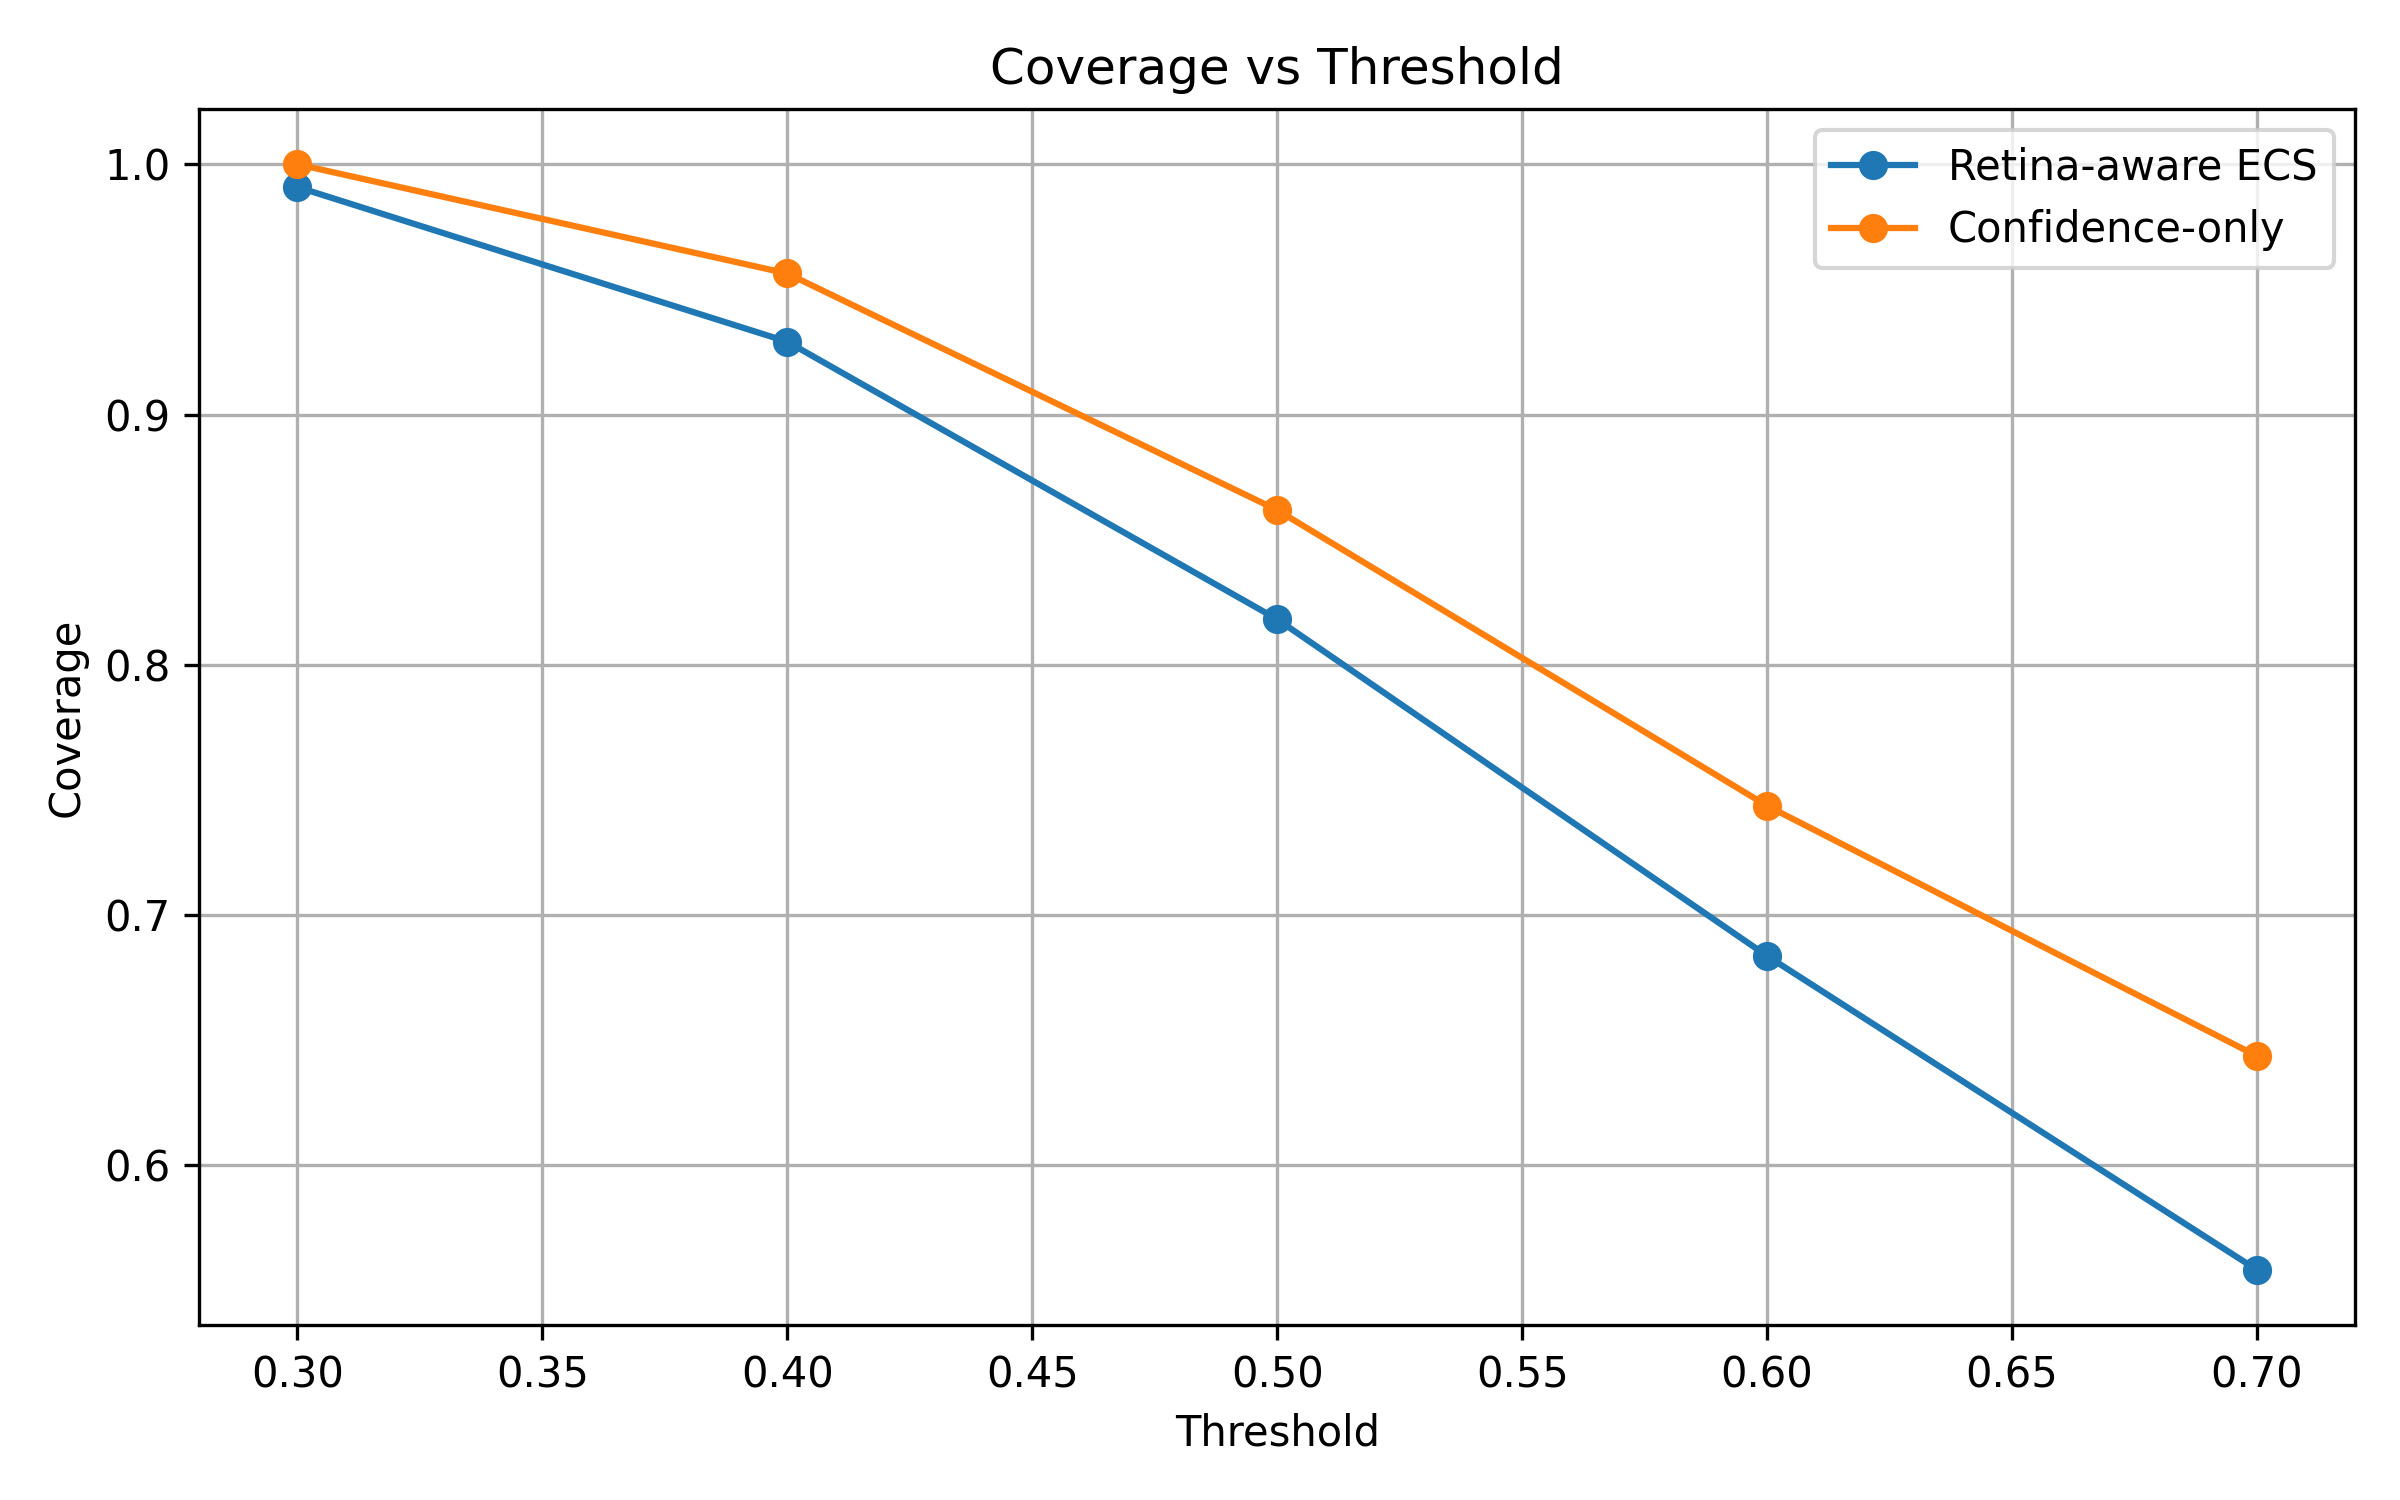
\includegraphics[width=\linewidth]{coverage_vs_threshold.png}
    \caption{Coverage as a function of threshold for retina-aware ECS and confidence-only selective prediction. Coverage decreases as the threshold becomes stricter.}
    \label{fig:coverage_threshold}
\end{figure}

\begin{figure}[!t]
    \centering
    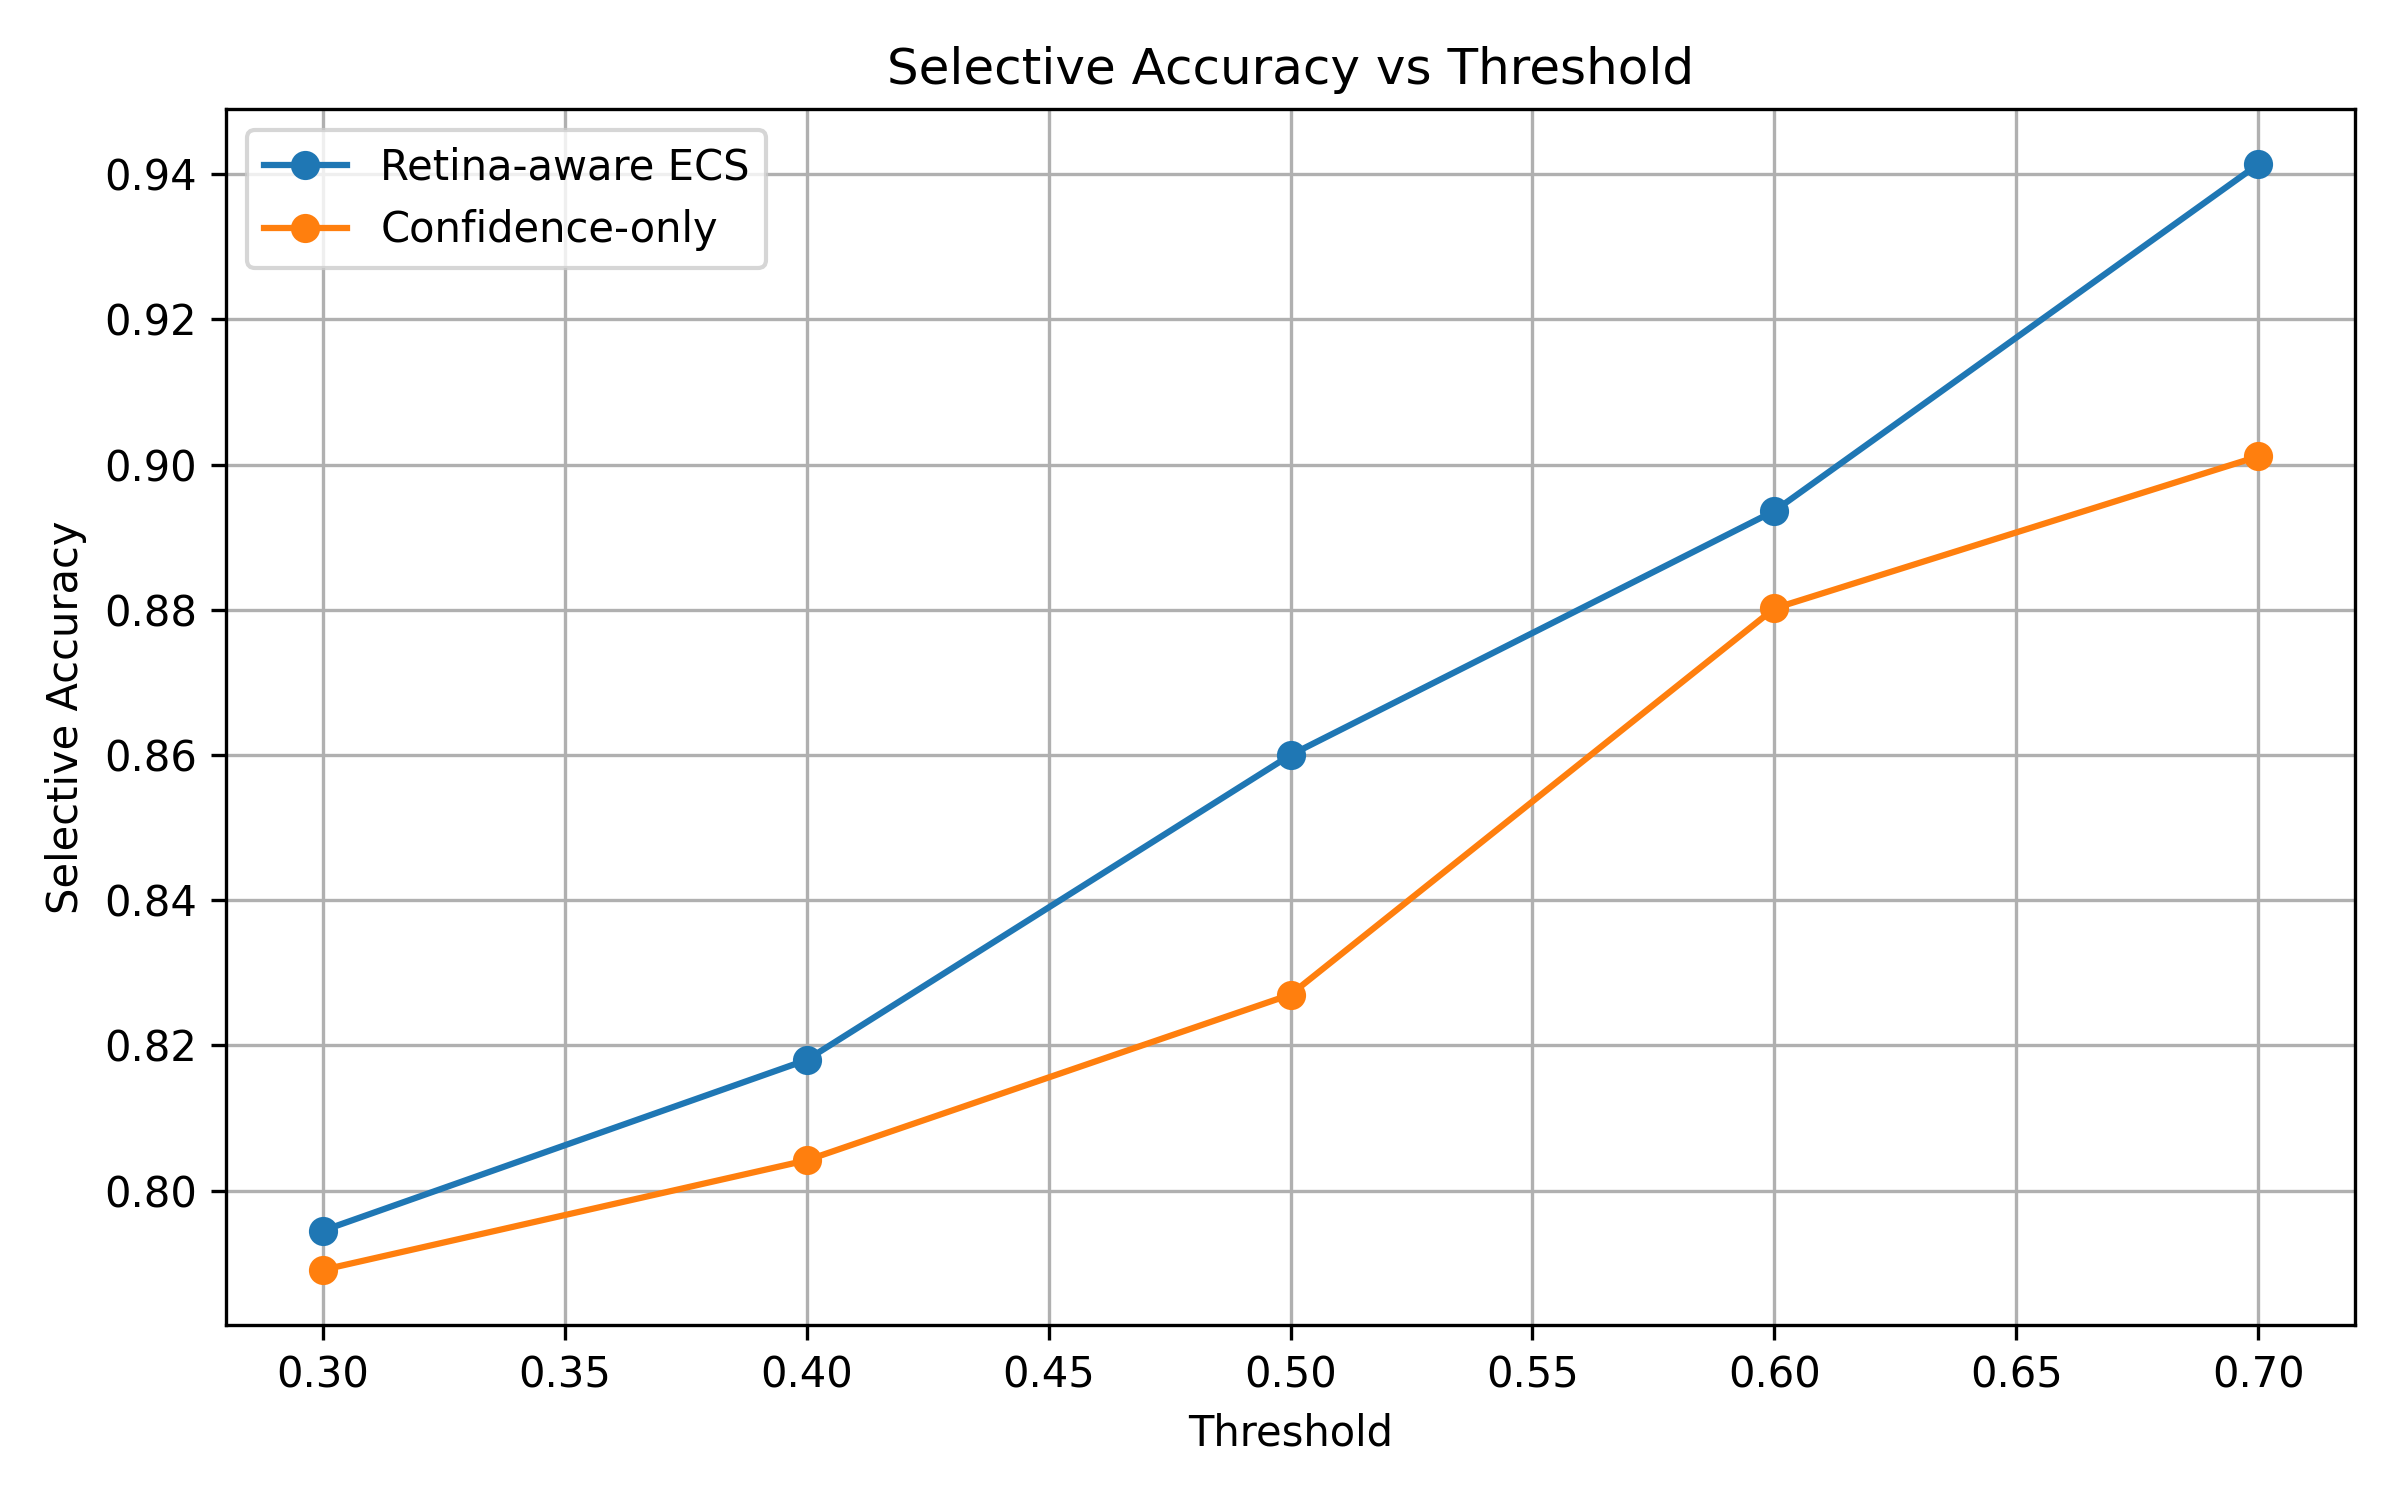
\includegraphics[width=\linewidth]{selective_accuracy_vs_threshold.png}
    \caption{Selective accuracy versus threshold. Retina-aware ECS consistently achieves higher selective accuracy than confidence-only selection across all evaluated thresholds.}
    \label{fig:acc_threshold}
\end{figure}

\subsection{Risk--Coverage Analysis}
The risk--coverage curve provides the clearest evidence of the advantage of the proposed method. Across the evaluated thresholds, retina-aware ECS consistently achieved lower risk than the confidence-only baseline at comparable coverage levels. This indicates that explanation-aware reliability estimation is more informative than raw confidence alone for determining which predictions are safe to accept.

From a practical perspective, this is highly relevant in medical AI settings. A confidence-only system may still accept cases with anatomically inconsistent attention patterns, whereas the proposed ECS explicitly penalizes such cases by incorporating retinal overlap and Grad-CAM focus.

\begin{figure}[!t]
    \centering
    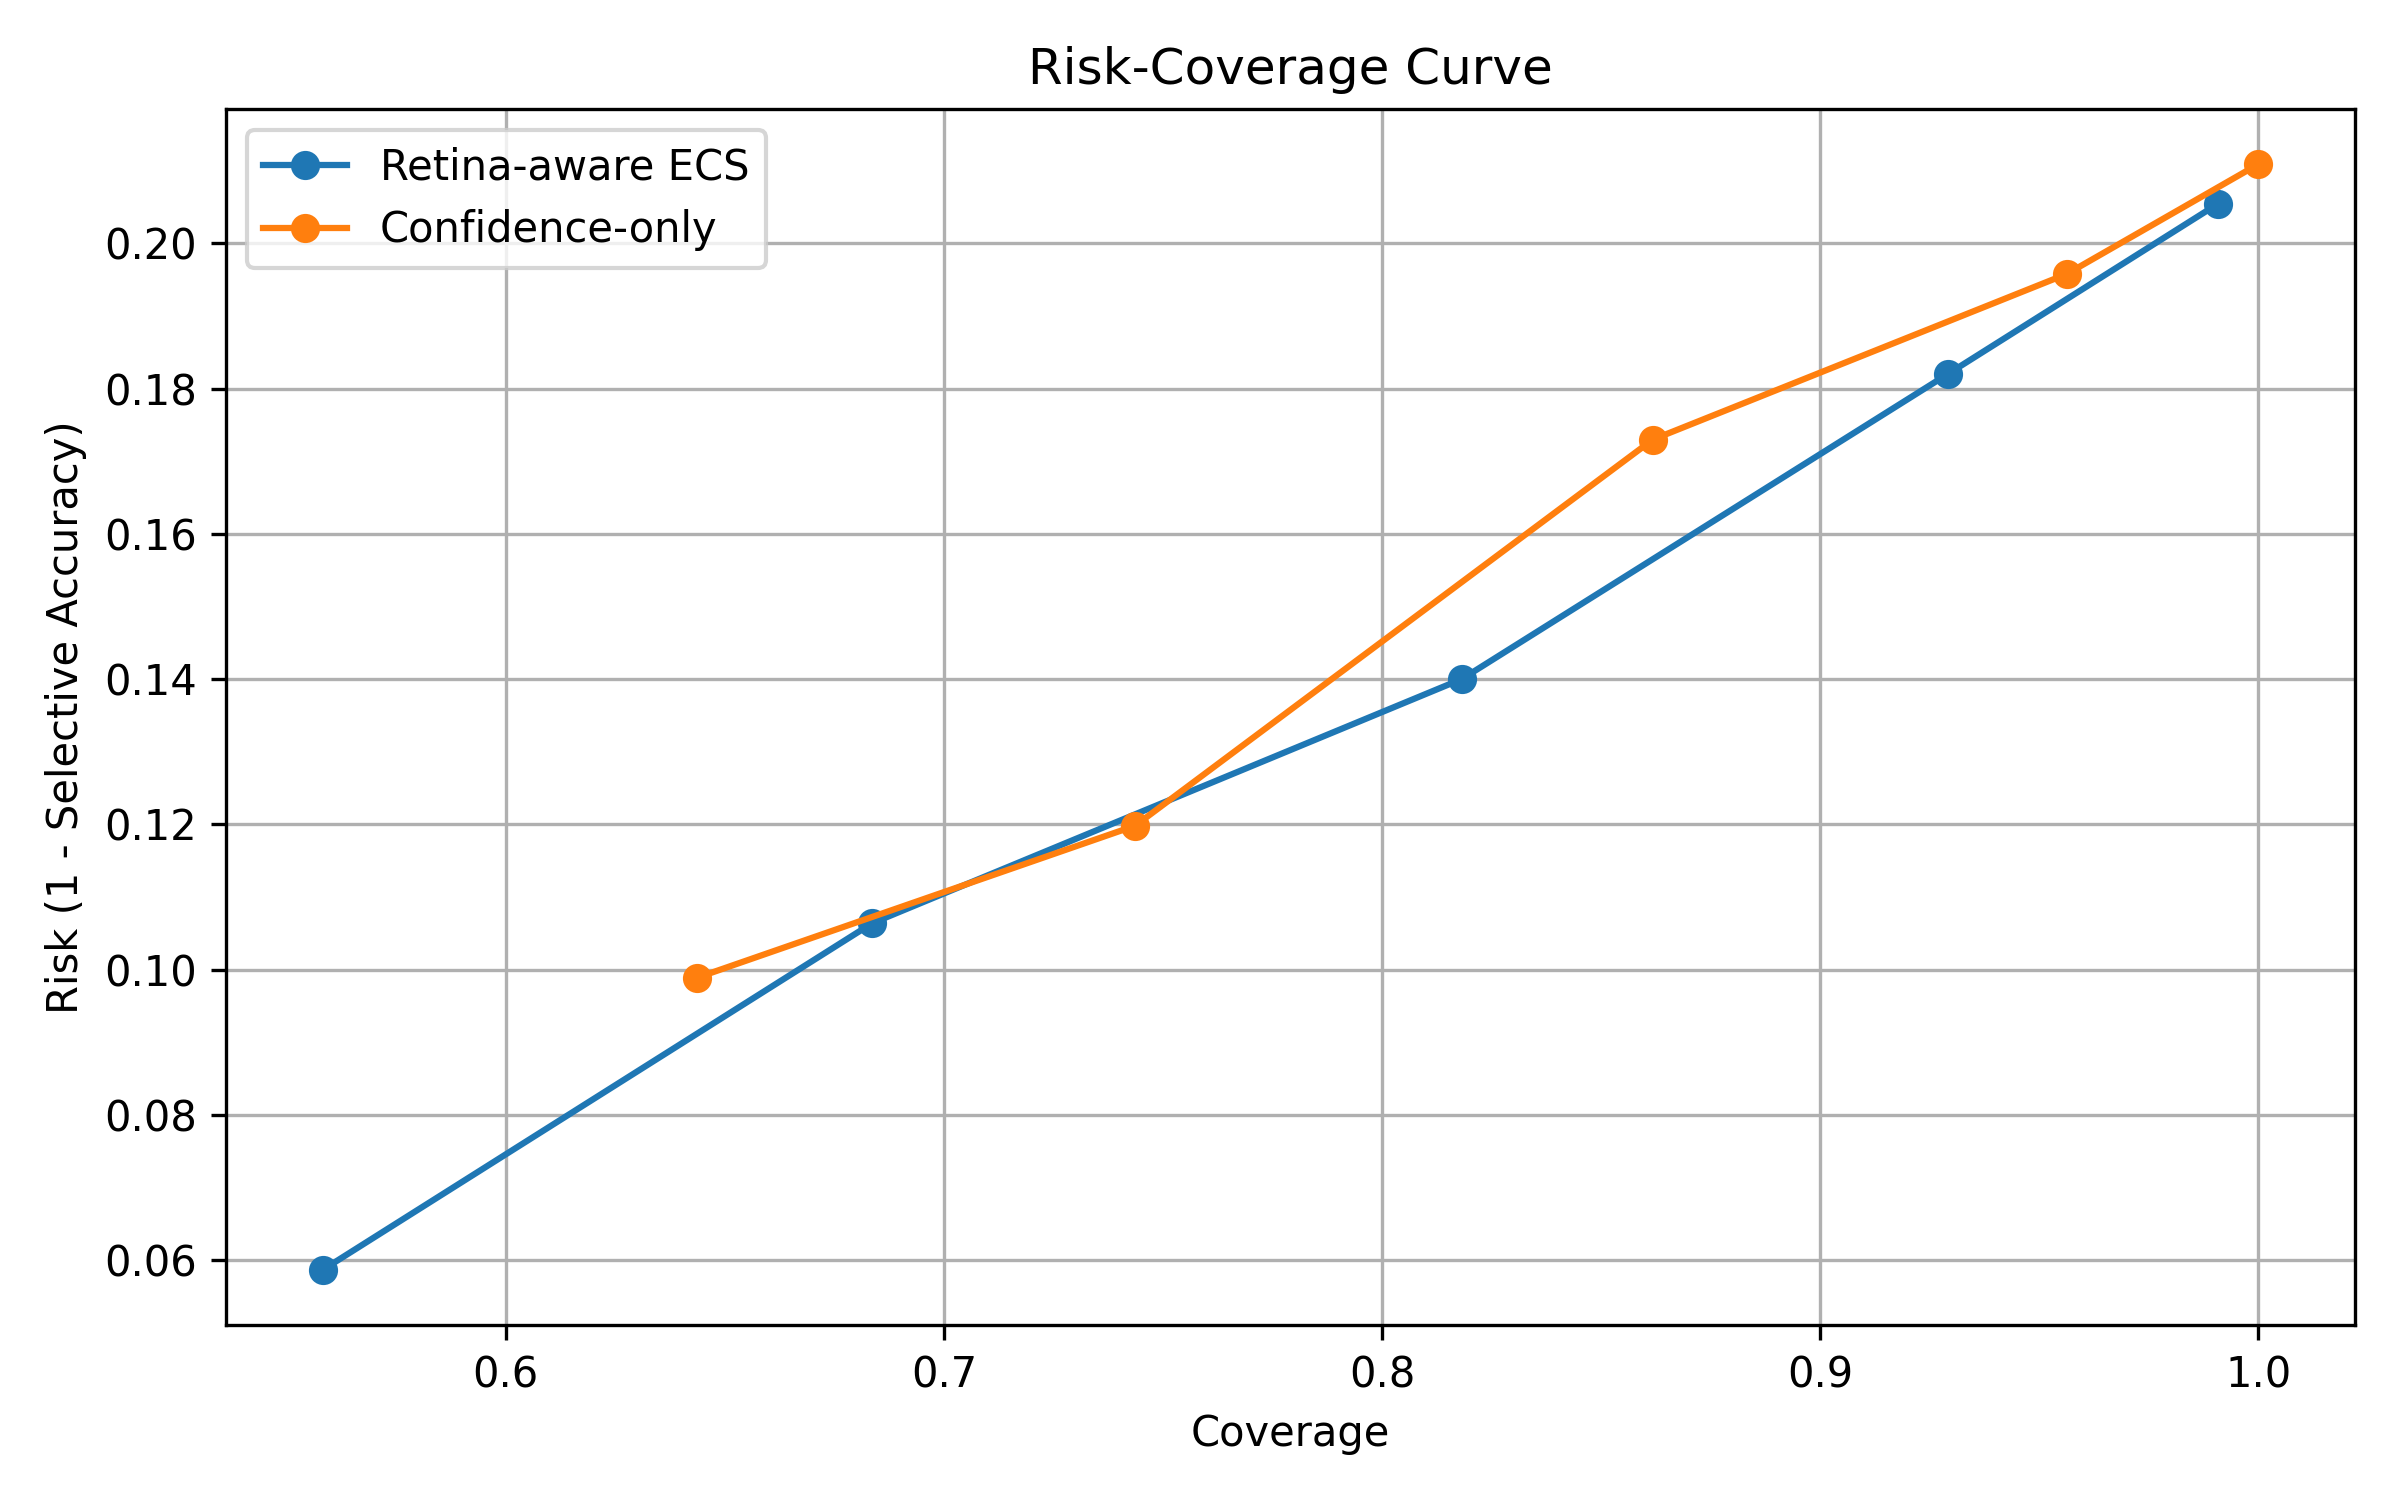
\includegraphics[width=\linewidth]{risk_coverage_curve.png}
    \caption{Risk--coverage curve for retina-aware ECS and confidence-only baseline. Lower risk at similar coverage indicates more reliable selective prediction.}
    \label{fig:risk_coverage}
\end{figure}

\subsection{Qualitative Grad-CAM Analysis}
The qualitative Grad-CAM results support the quantitative findings. In high-ECS cases, model attention remains concentrated within the retinal disc and aligns with visually meaningful retinal structures. In weaker cases, the activation patterns are more diffuse or less anatomically constrained. This suggests that integrating explanation quality into reliability estimation provides an additional safeguard beyond calibrated confidence alone.

\begin{figure}[!t]
    \centering
    \subfloat[Input]{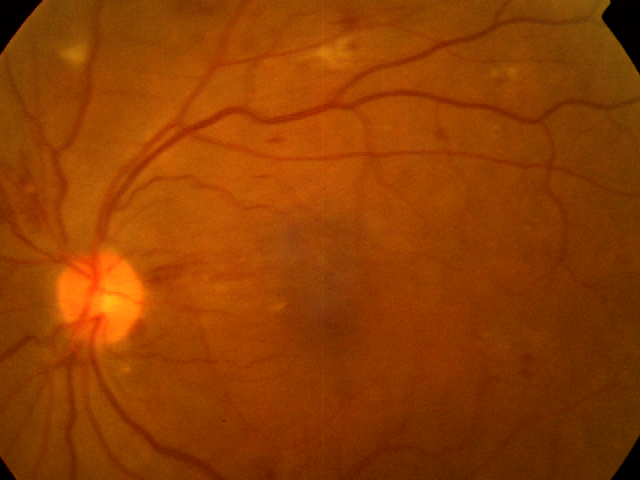
\includegraphics[width=0.22\linewidth]{normal_image_1.png}}
    \hfill
    \subfloat[Grad-CAM]{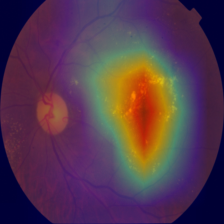
\includegraphics[width=0.22\linewidth]{heatmap_image_1.png}}
    \hfill
    \subfloat[Input]{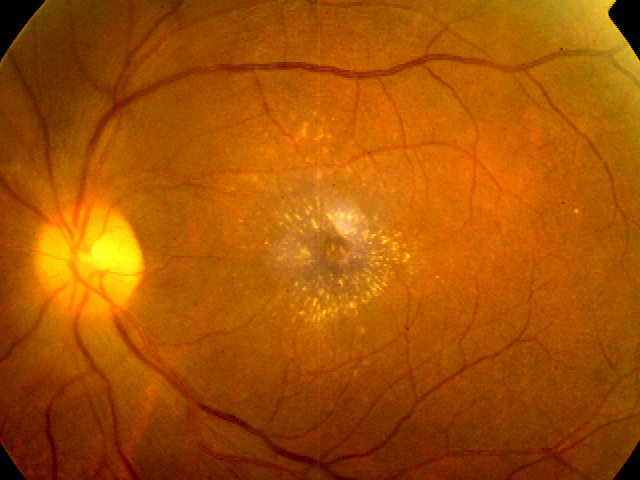
\includegraphics[width=0.22\linewidth]{normal_image_2.png}}
    \hfill
    \subfloat[Grad-CAM]{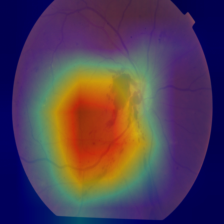
\includegraphics[width=0.22\linewidth]{heatmap_image_2.png}}
    \caption{Representative Grad-CAM examples for retinal fundus images. High-reliability cases show attention concentrated within anatomically valid retinal regions, whereas weaker cases exhibit less consistent spatial focus.}
    \label{fig:gradcam_examples}
\end{figure}

\subsection{Why Retina-Aware ECS Improves Reliability}
The proposed method is effective because it combines complementary reliability signals rather than depending on a single scalar quantity. Confidence captures the model’s belief in its own prediction, entropy captures uncertainty in the predictive distribution, Grad-CAM focus reflects localization sharpness, and retinal overlap introduces anatomical consistency.

This combination is particularly important in medical image analysis. A model can be confident for the wrong reason, and a visually sharp explanation is not necessarily trustworthy if it lies outside the anatomical region of interest. By filtering predictions using both probabilistic and spatial consistency criteria, the proposed framework produces a more reliable accepted subset.

\subsection{Practical Implications}
The proposed framework is relevant for real-world AI-assisted screening systems. In a deployment scenario, the model can automatically handle reliable cases while deferring low-ECS cases to human experts. Such a human-AI workflow is especially valuable in large-scale screening programs, where efficiency and safety must be balanced.

This makes the proposed method practical not only as a classification model, but also as a decision-support mechanism that provides a structured way to manage uncertainty.

\subsection{Limitations}
Despite its advantages, the current framework has several limitations. First, the retinal prior is based on anatomical masking rather than explicit lesion-level supervision. Second, Grad-CAM is a post-hoc explanation method and may not fully capture the entire internal reasoning process of the model. Third, the experiments were conducted on a single public dataset, and broader validation on additional retinal datasets would strengthen claims of generalization.

These limitations also suggest natural future directions, including lesion-aware overlap scoring, adaptive weighting of ECS components, cross-dataset validation, and extension to deep-ensemble ECS scoring.

\FloatBarrier
\section{Conclusion}
This paper presented a retina-aware reliability framework for diabetic retinopathy classification that combines calibration, explainability, and selective prediction. Beyond producing accurate class predictions, the proposed method explicitly evaluates whether a prediction is visually and anatomically trustworthy. The resulting Explanation Consistency Score integrates calibrated confidence, entropy, Grad-CAM focus, and retinal overlap into a unified reliability criterion.

Experimental results on the APTOS dataset show that temperature scaling improves calibration without changing classification accuracy, while retina-aware ECS consistently produces a more favorable risk--coverage trade-off than a confidence-only baseline. At practically relevant thresholds, the proposed framework yields more reliable accepted predictions and provides a stronger basis for trustworthy medical AI deployment.

Overall, this work demonstrates that moving beyond confidence-only reliability estimation is essential for safety-critical medical AI. By incorporating explainability and anatomical consistency, the proposed method offers a more meaningful notion of trustworthiness for retinal image classification systems.

\section*{Acknowledgment}
The authors would like to express their sincere gratitude to Dr. Sunil Datt Sharma, Associate Professor, Department of Electronics and Communication Engineering, Central University of Jammu, for his valuable guidance, mentorship, and continuous support throughout this research work.

\bibliographystyle{IEEEtran}
\bibliography{references}

\end{document}